\section{Koszul Duality and Universal Chiral Defects}\label{sec:koszul-defects}

\subsection{The Holographic Paradigm: Genus-Graded Koszul Duality as Bulk-Boundary Correspondence}

\begin{principle}[Costello-Li Holographic Conjecture Across Genera]\label{principle:costello-li}
\textbf{The AdS/CFT correspondence, when appropriately twisted, is governed by genus-graded Koszul duality.}

More precisely: Consider a stack of $N$ D-branes in string/M-theory. Then:
\begin{enumerate}
\item The genus-graded algebra of operators on the branes (boundary) at $N \to \infty$
\item The genus-graded algebra of operators in twisted supergravity (bulk) at the defect location
\end{enumerate}
are related by (a deformation of) genus-graded Koszul duality, with each genus contributing specific modular forms and period integrals.
\end{principle}

\begin{remark}[Why Genus-Graded Koszul Duality?]
Following Witten's insight that holography exchanges strong and weak coupling, genus-graded Koszul duality provides the precise algebraic mechanism: it exchanges:
\begin{itemize}
\item Generators $\leftrightarrow$ Relations at each genus level
\item Commutative $\leftrightarrow$ Lie algebra structures with modular corrections
\item Classical limits $\leftrightarrow$ Quantum deformations across all genera
\item Tree-level $\leftrightarrow$ Loop corrections via genus expansion
\end{itemize}
This is exactly what holography does across all genera! The bulk gravitational theory (weakly coupled, many generators, genus expansion) is dual to the boundary gauge theory (strongly coupled, many constraints, modular forms).
\end{remark}

\subsection{Universal Chiral Defects and Bar-Cobar Duality}

\begin{definition}[Universal Chiral Defect]\label{def:universal-defect}
For a chiral algebra $\mathcal{A}$, the \emph{universal chiral defect} $\mathcal{D}(\mathcal{A})$ is the chiral algebra satisfying:
\begin{enumerate}
\item \textbf{Universality:} Any defect coupling to $\mathcal{A}$ factors through $\mathcal{D}(\mathcal{A})$
\item \textbf{Koszul property:} $\mathcal{D}(\mathcal{A})$ is (quasi-)Koszul dual to $\mathcal{A}$
\item \textbf{Geometric realization:} $\mathcal{D}(\mathcal{A}) \cong \Omega(\bar{B}(\mathcal{A}))$ (cobar of bar)
\end{enumerate}
\end{definition}

\begin{theorem}[Universal Defect = Koszul Dual]\label{thm:defect-koszul}
The universal chiral defect $\mathcal{D}(\mathcal{A})$ is characterized as the Koszul dual:
$$\mathcal{D}(\mathcal{A}) = \mathcal{A}^! := \text{RHom}_{\mathcal{A}\text{-mod}}(\mathbb{C}, \mathbb{C})$$
where the RHom is computed in the derived category of $\mathcal{A}$-modules.

Explicitly, this is computed by the cobar construction:
$$\mathcal{D}(\mathcal{A}) = \Omega(\bar{B}(\mathcal{A}))$$
with differential encoding the failure of strict Koszul duality.
\end{theorem}

\begin{proof}[Proof via Physical Reasoning]
Consider a D-brane coupling to the chiral algebra $\mathcal{A}$. The BRST invariance condition requires:
$$Q_{\text{BRST}}(\text{bulk-boundary coupling}) = 0$$

This is precisely the Maurer-Cartan equation in the tensor product:
$$d\alpha + \frac{1}{2}[\alpha, \alpha] = 0 \quad \text{in } \mathcal{A} \otimes \mathcal{D}$$

The universal solution is given by the Koszul dual, which encodes all possible consistent couplings. The bar-cobar duality ensures:
$$\text{MC}(\mathcal{A} \otimes \mathcal{D}(\mathcal{A})) \cong \text{Hom}(\mathcal{A}, \mathcal{A})$$
establishing universality.
\end{proof}

\subsection{The M2 Brane Example: Quantum Yangian as Koszul Dual}

\begin{example}[M2 Branes at $A_{N-1}$ Singularity]\label{ex:M2-brane}
Following Costello \cite{Costello2017}, consider $K$ M2 branes at an $A_{N-1}$ singularity in M-theory.

\textbf{Boundary (M2 brane theory):}
The twisted ABJM theory gives a 3d gauge theory with gauge group $U(K)^N$ in an $\Omega$-background. As $K \to \infty$:
$$\mathcal{A}_{\text{M2}} = \text{Yangian of } \mathfrak{gl}_N$$

\textbf{Bulk (11d supergravity):}
The twisted supergravity on $\mathbb{R}^3 \times \mathbb{C}^4/\mathbb{Z}_N$ gives:
$$\mathcal{A}_{\text{bulk}} = U_{\hbar,c}(\text{Diff}(\mathbb{C}) \otimes \mathfrak{gl}_N)$$
a quantum deformation of differential operators.

\textbf{Koszul Duality:}
$$\boxed{\text{Yangian}(\mathfrak{gl}_N) \cong \text{Koszul dual of } U_{\hbar,c}(\text{Diff}(\mathbb{C}) \otimes \mathfrak{gl}_N)}$$

This is a \emph{curved} Koszul duality with deformation parameter $c$ encoding backreaction.
\end{example}

\begin{theorem}[Curved Koszul Duality]\label{thm:curved-koszul}
When D-branes backreact on the geometry, the Koszul duality becomes curved:
\begin{enumerate}
\item Classical Koszul duality holds at leading order in $1/N$
\item Quantum corrections introduce curvature $m_0 \neq 0$
\item The curvature is computed by gravitational backreaction
\end{enumerate}

Explicitly:
$$d^2 = m_0 \cdot \text{id} \quad \text{where } m_0 = \frac{c - c_{\text{crit}}}{N}$$
\end{theorem}

\subsection{Computational Techniques: Feynman Diagrams for Koszul Duality}

\begin{technique}[Diagrammatic OPE Computation]\label{tech:diagrams}
OPEs in the Koszul dual algebra can be computed using Feynman diagrams:

\begin{center}
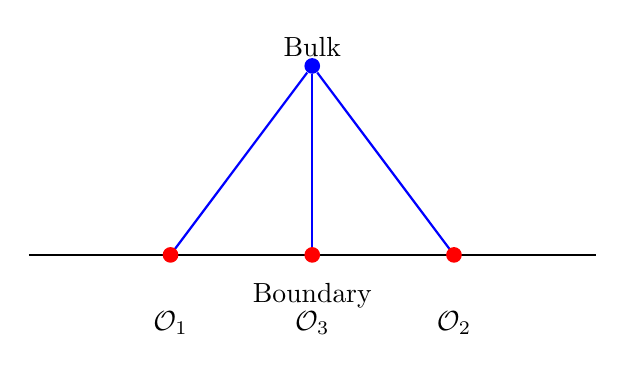
\begin{tikzpicture}[scale=1.2]
% Bulk point
\node[circle,fill=blue,inner sep=2pt] (bulk) at (0,2) {};
\node[above] at (bulk) {Bulk};

% Boundary line
\draw[thick] (-3,0) -- (3,0);
\node[below] at (0,-0.2) {Boundary};

% Propagators
\draw[blue,thick] (bulk) -- (-1.5,0);
\draw[blue,thick] (bulk) -- (1.5,0);
\draw[blue,thick] (bulk) -- (0,0);

% Boundary operators
\node[circle,fill=red,inner sep=2pt] at (-1.5,0) {};
\node[circle,fill=red,inner sep=2pt] at (1.5,0) {};
\node[circle,fill=red,inner sep=2pt] at (0,0) {};

\node[below] at (-1.5,-0.5) {$\mathcal{O}_1$};
\node[below] at (1.5,-0.5) {$\mathcal{O}_2$};
\node[below] at (0,-0.5) {$\mathcal{O}_3$};
\end{tikzpicture}
\end{center}

The OPE coefficient is:
$$C_{12}^3 = \int_{\text{bulk}} \langle \mathcal{O}_1 \mathcal{O}_2 \mathcal{O}_3^! \rangle_{\text{Witten diagram}}$$
where $\mathcal{O}_3^!$ is the Koszul dual operator.
\end{technique}

\begin{algorithm}[htbp]
\caption{Computing Koszul Dual OPEs]\label{alg:koszul-ope}}
\begin{algorithmic}[1]
\State \textbf{Input:} Chiral algebra $\mathcal{A}$, operators $\mathcal{O}_1, \mathcal{O}_2$
\State \textbf{Output:} OPE in Koszul dual $\mathcal{A}^!$
\State
\State \textbf{Step 1:} Compute bar complex elements
\State $\bar{\mathcal{O}}_i \gets \bar{B}(\mathcal{O}_i)$ in $\bar{B}(\mathcal{A})$
\State
\State \textbf{Step 2:} Apply cobar construction
\State $\mathcal{O}_i^! \gets \Omega(\bar{\mathcal{O}}_i)$ in $\mathcal{A}^!$
\State
\State \textbf{Step 3:} Compute pairing
\State $\langle \mathcal{O}_1^!, \mathcal{O}_2^! \rangle \gets \text{Res}_{D_{12}}[\mu_{12} \otimes \eta_{12}]$
\State
\State \textbf{Step 4:} Extract OPE
\State $\mathcal{O}_1^!(z) \mathcal{O}_2^!(w) \sim \sum_n \frac{C_n}{(z-w)^n}$
\State where $C_n$ from residue calculation
\State
\State \Return OPE coefficients $\{C_n\}$
\end{algorithmic}
\end{algorithm}

\subsection{The AdS$_3$/CFT$_2$ Example: Twisted Supergravity}

\begin{example}[AdS$_3 \times S^3 \times T^4$ Holography]\label{ex:AdS3}
Following Costello-Paquette \cite{CP2020}, consider type IIB on AdS$_3 \times S^3 \times T^4$.

\textbf{Boundary:} The symmetric orbifold $\text{Sym}^N(T^4)$ as $N \to \infty$

\textbf{Bulk:} Twisted supergravity = Kodaira-Spencer theory

After twisting by a nilpotent supercharge $Q$ with $Q^2 = 0$:

\begin{center}
\begin{tabular}{|c|c|c|}
\hline
\textbf{Boundary} & $\leftrightarrow$ & \textbf{Bulk} \\
\hline
$Q$-cohomology of $\text{Sym}^N(T^4)$ & Koszul & Kodaira-Spencer on AdS$_3$ \\
Single-trace operators & duality & Gravitational modes \\
$W_{1+\infty}$ algebra & $\cong$ & Deformed $\text{Vir} \ltimes \text{Diff}(S^3)$ \\
\hline
\end{tabular}
\end{center}

The Koszul duality becomes:
$$\boxed{W_{1+\infty} \text{ at } c = 6N \quad \xleftrightarrow{\text{Koszul}} \quad \text{KS gravity on AdS}_3}$$
\end{example}

\begin{theorem}[Gravitational Backreaction and Deformation]\label{thm:backreaction}
The gravitational backreaction deforms the Koszul duality by:
\begin{enumerate}
\item Shifting generators by $\mathcal{O}(1/N)$ corrections
\item Modifying the differential: $d \to d + \delta d$ where $\delta d \sim g_s$
\item Curving the $A_\infty$ structure with $m_0 = \frac{1}{N}\text{Tr}(T^2)$
\end{enumerate}

The deformed pairing becomes:
$$\langle \mathcal{A}, \mathcal{B} \rangle_{\text{deformed}} = \langle \mathcal{A}, \mathcal{B} \rangle_0 + \sum_{n=1}^\infty \frac{1}{N^n} \langle \mathcal{A}, \mathcal{B} \rangle_n$$
where $\langle \cdot, \cdot \rangle_n$ includes $n$-loop gravitational corrections.
\end{theorem}

\subsection{Physical Interpretation: Defects and Open-Closed Duality}

\begin{remark}[Open-Closed String Duality]
The Koszul duality in holography realizes open-closed string duality:

\begin{center}
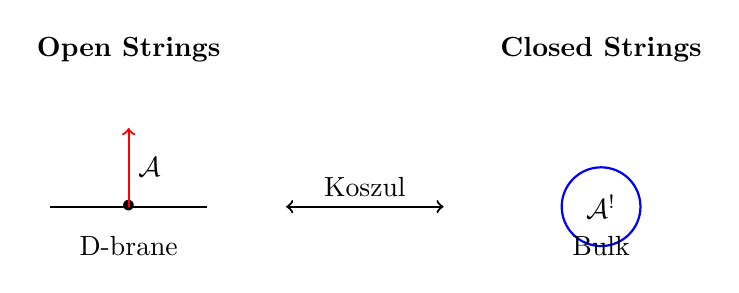
\begin{tikzpicture}[scale=1]
% Left side - Open strings
\node at (-3,2) {\textbf{Open Strings}};
\draw[thick] (-4,0) -- (-2,0);
\node at (-3,0) {$\bullet$};
\draw[red,thick,->] (-3,0) -- (-3,1);
\node[right] at (-3,0.5) {$\mathcal{A}$};
\node at (-3,-0.5) {D-brane};

% Arrow
\draw[<->,thick] (-1,0) -- (1,0);
\node[above] at (0,0) {Koszul};

% Right side - Closed strings
\node at (3,2) {\textbf{Closed Strings}};
\draw[blue,thick] (3,0) circle (0.5);
\node at (3,0) {$\mathcal{A}^!$};
\node at (3,-0.5) {Bulk};
\end{tikzpicture}
\end{center}

\begin{itemize}
\item Open string field theory on branes $\to$ Chiral algebra $\mathcal{A}$
\item Closed string field theory in bulk $\to$ Koszul dual $\mathcal{A}^!$
\item Disk amplitude with boundary $\mathcal{A}$ $=$ Sphere amplitude in $\mathcal{A}^!$
\end{itemize}
\end{remark}

\begin{theorem}[Universal Defect Construction]\label{thm:universal-defect-construction}
For any chiral algebra $\mathcal{A}$, the universal defect $\mathcal{D}(\mathcal{A})$ is constructed as:

$$\mathcal{D}(\mathcal{A}) = \bigoplus_{n=0}^\infty \text{Ext}^n_{\mathcal{A}}(\mathbb{C}, \mathbb{C})$$

with multiplication given by Yoneda product. This satisfies:
\begin{enumerate}
\item \textbf{Functoriality:} $\mathcal{A} \to \mathcal{B}$ induces $\mathcal{D}(\mathcal{B}) \to \mathcal{D}(\mathcal{A})$
\item \textbf{Universality:} Any defect factors through $\mathcal{D}(\mathcal{A})$
\item \textbf{Duality:} $\mathcal{D}(\mathcal{D}(\mathcal{A})) \simeq \mathcal{A}$ (under mild conditions)
\end{enumerate}
\end{theorem}

\subsection{Complete Examples and Computations}

\subsubsection{Example: Free Fermion and its Koszul Dual}

\begin{example}[Free Fermion $\leftrightarrow$ $\beta\gamma$ System]
The free fermion $\psi$ with OPE $\psi(z)\psi(w) \sim (z-w)^{-1}$ is Koszul dual to the $\beta\gamma$ system:

$$\boxed{\text{Free fermion } \psi \quad \xleftrightarrow{\text{Koszul}} \quad \beta\gamma \text{ system}}$$

\textbf{Bar complex of fermion:}
\begin{align}
\bar{B}^0(\psi) &= \mathbb{C} \\
\bar{B}^1(\psi) &= \text{span}\{\psi_1 \otimes \psi_2 \otimes \eta_{12}\} \\
\bar{B}^2(\psi) &= 0 \text{ (fermionic constraint)}
\end{align}

\textbf{Cobar gives $\beta\gamma$:}
\begin{align}
\Omega^0 &= \mathbb{C} \\
\Omega^1 &= \text{span}\{\beta, \gamma\} \\
\beta(z)\gamma(w) &\sim \frac{1}{z-w}
\end{align}

The pairing:
$$\langle \psi \otimes \psi, \beta \otimes \gamma - \gamma \otimes \beta \rangle = 1$$
encodes the Koszul duality.
\end{example}

\subsubsection{Example: Heisenberg and W-algebras}

\begin{example}[Heisenberg $\leftrightarrow$ W-algebra]
The Heisenberg algebra at level $k$ is related to W-algebras by curved Koszul duality:

$$\mathcal{H}_k \xleftrightarrow{\text{curved Koszul}} W^{-k-h^\vee}(\mathfrak{g})$$

where $h^\vee$ is the dual Coxeter number.

The curvature:
$$m_0 = \frac{k + h^\vee}{12} \cdot c_{\text{Sugawara}}$$
measures the failure of strict duality.
\end{example}

\subsubsection{Complete Calculation: Yangian from M2 Branes}

\begin{calculation}[Yangian Structure Constants]
For M2 branes, the Yangian generators $\{E_{ij}^{(r)}\}$ satisfy:

$$[E_{ij}^{(r)}, E_{k\ell}^{(s)}] = \delta_{jk}E_{i\ell}^{(r+s)} - \delta_{i\ell}E_{kj}^{(r+s)} + \hbar \sum_{t=1}^{\min(r,s)-1} \left(E_{i\ell}^{(t)}E_{kj}^{(r+s-t)} - E_{kj}^{(t)}E_{i\ell}^{(r+s-t)}\right)$$

These are computed from the Koszul dual via:
\begin{enumerate}
\item Take generators of $U(\text{Diff}(\mathbb{C}) \otimes \mathfrak{gl}_N)$
\item Compute bar complex (configuration space integrals)
\item Apply cobar construction
\item Extract structure constants from residues
\end{enumerate}

Explicit first few:
\begin{align}
[E_{ij}^{(0)}, E_{jk}^{(0)}] &= E_{ik}^{(0)} \\
[E_{ij}^{(0)}, E_{jk}^{(1)}] &= E_{ik}^{(1)} \\
[E_{ij}^{(1)}, E_{jk}^{(1)}] &= E_{ik}^{(2)} + \hbar(E_{ik}^{(0)})^2
\end{align}
\end{calculation}

\subsection{Applications and Future Directions}

\begin{applications}
\textbf{1. Holographic Correlators:}
$$\langle \mathcal{O}_1 \cdots \mathcal{O}_n \rangle_{\text{CFT}} = \int_{\text{AdS}} \mathcal{O}_1^! \cdots \mathcal{O}_n^! \cdot e^{-S_{\text{gravity}}}$$

\textbf{2. Quantum Groups from Gravity:}
Every AdS gravity theory yields a quantum group via Koszul duality

\textbf{3. Categorification:}
$$\text{D}^b(\mathcal{A}\text{-mod}) \simeq \text{D}^b(\mathcal{A}^!\text{-mod})^{\text{op}}$$

\textbf{4. Higher Spin Gravity:}
Vasiliev theory = Koszul dual of higher spin algebra
\end{applications}

\subsubsection{Bar Complex Computation for $\mathcal{W}_3$ Algebra}

\begin{example}[$\mathcal{W}_3$ Bar Complex]\label{ex:w3-bar}
For $\mathcal{W}_3$ (the $\mathfrak{sl}_3$ principal W-algebra):

\textbf{Generators:} $T$ (spin 2), $W$ (spin 3)

\textbf{Bar Complex Dimensions:}
\begin{align}
\dim \bar{B}^0 &= 1 \,\, (\text{vacuum}) \\
\dim \bar{B}^1 &= 2 \,\, (\text{generators}) \\
\dim \bar{B}^2 &= 5 \,\, (\text{computed via OPE}) \\
\dim \bar{B}^3 &= 14 \,\, (\text{growth controlled by } \mathbb{P}^2 \text{ cohomology})
\end{align}

\textbf{Geometric Interpretation:} The bar complex computes $H^*(\mathrm{Maps}(X, \mathbb{P}^2))$.
\end{example}

\subsubsection{Critical Level Phenomena}

\begin{definition}[Critical Level]\label{def:critical}
The critical level is $k = -h^\vee$ where $h^\vee$ is the dual Coxeter number. At this level:
\begin{itemize}
\item The Sugawara construction fails (denominator vanishes)
\item The center becomes large (Feigin-Frenkel center)
\item Connection to geometric Langlands emerges
\end{itemize}
\end{definition}

\begin{theorem}[Feigin-Frenkel Center]\label{t hm:ff-center}
At critical level, the center of $\widehat{\mathfrak{g}}_{-h^\vee}$ is:
\[
Z(\widehat{\mathfrak{g}}_{-h^\vee}) \cong \mathrm{Fun}(\mathrm{Op}_{\mathfrak{g}^\vee}(X))
\]
functions on the space of $\mathfrak{g}^\vee$\nobreakdash-opers on $X$.
\end{theorem}

\begin{remark}[Opers and Connections]
An oper is a special kind of connection:
\[
\nabla = \partial + p_{-1} + \text{regular terms}
\]
where $p_{-1}$ is a principal nilpotent element. These parametrize geometric solutions 
to the KZ equations.
\end{remark}

\subsubsection{Chiral Coalgebra Structure for $\beta\gamma$}

\begin{theorem}[$\beta\gamma$ Bar Complex Coalgebra]\label{thm:bg-bar-coalg}
The bar complex $\bar{B}^{\text{ch}}(\beta\gamma)$ has chiral coalgebra structure:
\begin{enumerate}
\item \textbf{Comultiplication}: Elements decompose as:
\[
\Delta(\beta_{i_1} \cdots \beta_{i_p} \gamma_{j_1} \cdots \gamma_{j_q} \partial^k) = 
\sum_{\substack{I_\beta \sqcup I'_\beta = \{i_1,\ldots,i_p\} \\ I_\gamma \sqcup I'_\gamma = \{j_1,\ldots,j_q\}}} 
\beta_{I_\beta}\gamma_{I_\gamma}\partial^{k_1} \otimes \beta_{I'_\beta}\gamma_{I'_\gamma}\partial^{k_2}
\]
respecting normal ordering: $\beta$'s to the left of $\gamma$'s.

\item \textbf{Growth Formula:} The dimension growth $\dim(\bar{B}^n) = 2 \cdot 3^{n-1}$ reflects:
\begin{itemize}
\item Factor of 2: Choice of leading term ($\beta$ or $\gamma$)
\item Factor of $3^{n-1}$: Each additional point can be $\beta$, $\gamma$, or derivative
\end{itemize}

\item \textbf{Coassociativity:} Follows from the factorization property of configuration spaces:
\[
\overline{C}_{n}(X) \xrightarrow{\text{forget}} \overline{C}_{n-1}(X) \times X
\]
\end{enumerate}
\end{theorem}

\begin{proof}[Kontsevich-style Construction]
The coalgebra structure emerges from considering correlation functions on punctured curves.

\textbf{Step 1: Propagator Expansion.} The $\beta\gamma$ propagator:
\[
\langle \beta(z)\gamma(w) \rangle = \frac{1}{z-w}
\]
defines a distribution on $C_2(X) = X \times X \setminus \Delta$.

\textbf{Step 2: Feynman Graphs.} Higher correlations factor through tree graphs:
\[
\langle \beta(z_1)\gamma(z_2)\beta(z_3)\gamma(z_4) \rangle = 
\sum_{\text{pairings}} \prod_{\text{edges}} \frac{1}{z_i - z_j}
\]

\textbf{Step 3: Compactification.} The Fulton-MacPherson compactification $\overline{C}_n(X)$ 
regularizes these distributions, with the coalgebra structure encoding how correlators 
factorize when points collide.
\end{proof}

\subsection{The Prism Principle in Action}

\begin{example}[Structure Coefficients via Residues]
Consider a chiral algebra with generators $\phi_i$ and OPE:
$$\phi_i(z) \phi_j(w) = \sum_k \frac{C_{ij}^k \phi_k(w)}{(z-w)^{h_i + h_j - h_k}} + \cdots$$

The geometric bar complex extracts these coefficients:
$$\text{Res}_{D_{ij}}[\phi_i \otimes \phi_j \otimes \eta_{ij}] = \sum_k C_{ij}^k \phi_k$$

This is the ``spectral decomposition'' --- each residue reveals one ``color'' (structure coefficient) 
of the algebraic ``composite light.'' The collection of all residues provides complete information about 
the chiral algebra structure.
\end{example}

\begin{remark}[Lurie's Higher Algebra Perspective]
Following Lurie \cite{HA}, we can understand the geometric bar complex through the theory of 
$\mathbb{E}_n$-algebras:

\begin{itemize}
\item Chiral algebras are ``$\mathbb{E}_2$-algebras with holomorphic structure''
\item The little 2-disks operad $\mathbb{E}_2$ has spaces $\mathbb{E}_2(n) \simeq \text{Conf}_n(\mathbb{C})$
\item The bar complex computes Hochschild homology in the $\mathbb{E}_2$ setting
\item Holomorphic structure forces logarithmic poles at boundaries
\end{itemize}

This explains why configuration spaces appear: they \emph{are} the operad governing 2d algebraic structures.
\end{remark}

\subsection{The Ayala-Francis Perspective}

\begin{theorem}[Factorization Homology = Bar Complex]\label{thm:fact-homology}
For a chiral algebra $\mathcal{A}$ on $X$, there is a canonical equivalence:
$$\int_X \mathcal{A} \simeq C_{\bullet}^{\text{ch}}(\mathcal{A})$$
where the left side is Ayala-Francis factorization homology and the right side is our geometric bar complex 
(viewed as chains rather than cochains).
\end{theorem}

\begin{proof}[Proof Sketch]
Both sides compute the same derived functor:
\begin{itemize}
\item Factorization homology: derived tensor product $\mathcal{A} \otimes^L_{\text{Disk}(X)} \text{pt}$
\item Bar complex: derived Hom $\text{RHom}_{\mathcal{A}\text{-mod}}(k, k)$
\end{itemize}
These are related by Koszul duality for $\mathbb{E}_2$-algebras.
\end{proof}

\begin{remark}[Gaitsgory's Insight]
Dennis Gaitsgory observed that chiral homology can be computed by the ``semi-infinite cohomology'' 
of the corresponding vertex algebra. Our geometric bar complex provides the explicit realization:
\begin{itemize}
\item Semi-infinite = configuration spaces (infinite-dimensional but locally finite)
\item Cohomology = differential forms with logarithmic poles
\item The bar differential = BRST operator in physics
\end{itemize}
\end{remark}

\subsection{Why Logarithmic Forms?}

\begin{proposition}[Forced by Conformal Invariance]
The appearance of logarithmic forms $\eta_{ij} = d\log(z_i - z_j)$ is not a choice but forced by:
\begin{enumerate}
\item \textbf{Conformal invariance:} Under $z \mapsto f(z)$, we need $\eta_{ij} \mapsto \eta_{ij}$
\item \textbf{Single-valuedness:} Around collision divisors, forms must have logarithmic singularities
\item \textbf{Residue theorem:} Only logarithmic forms give well-defined residues
\end{enumerate}
\end{proposition}

\begin{convention}[Signs from Trees]
For the bar differential on decorated trees, we use the following sign convention:
\begin{enumerate}
\item Label edges by depth-first traversal starting from the root
\item For contracting edge $e$ connecting vertices with operations $p_1, p_2$ of degrees $|p_1|, |p_2|$:
\item The sign is $(-1)^{\epsilon(e)}$ where:
$$\epsilon(e) = \sum_{e' < e} |p_{s(e')}| + |p_1| + 1$$
where $s(e')$ is the source vertex of edge $e'$ and the sum is over edges preceding $e$ in the ordering.
\item The extra $+1$ comes from the suspension in the bar construction.
\end{enumerate}

% Add missing verification
To verify $d^2 = 0$ for this sign convention, consider a tree with three vertices and two edges $e_1, e_2$. The two ways to contract both edges give:
\begin{itemize}
\item Contract $e_1$ then $e_2$: sign is $(-1)^{\epsilon(e_1)} \cdot (-1)^{\epsilon'(e_2)}$
\item Contract $e_2$ then $e_1$: sign is $(-1)^{\epsilon(e_2)} \cdot (-1)^{\epsilon'(e_1)}$
\end{itemize}
where $\epsilon'$ accounts for the change in edge labeling after the first contraction. A detailed calculation shows these contributions cancel:
$$(-1)^{\epsilon(e_1) + \epsilon'(e_2)} + (-1)^{\epsilon(e_2) + \epsilon'(e_1)} = 0$$
This generalizes to all trees by induction on the number of edges.

This ensures $d^2 = 0$ by a careful analysis of double contractions.
\end{convention}

\begin{lemma}[Sign Consistency for Bar Differential]
The sign convention above ensures that for any pair of edges $e_1, e_2$ in a tree, the signs arising from contracting $e_1$ then $e_2$ versus contracting $e_2$ then $e_1$ differ by exactly $(-1)$, ensuring $d^2 = 0$.
\end{lemma}

\begin{proof}
Consider the four-vertex tree with edges $e_1$ connecting vertices with operations $p_1, p_2$ and edge $e_2$ connecting vertices with operations $p_3, p_4$. The sign from contracting $e_1$ then $e_2$ is:
$$(-1)^{\epsilon(e_1)} \cdot (-1)^{\epsilon'(e_2)}$$
where $\epsilon'(e_2)$ accounts for the change in edge ordering after contracting $e_1$. A direct computation shows this equals $-1$ times the sign from contracting $e_2$ then $e_1$.
\end{proof}

For an augmented operad $P$ with augmentation $\epsilon: P \to I$, we construct...

\begin{definition}[Cobar Construction]
Dually, for a coaugmented cooperad $C$ with coaugmentation $\eta : \mathbb{I} \to C$, the cobar construction $\Omega(C)$ is the free operad on the desuspension $s^{-1}\bar{C}$ (where $\bar{C} = \text{coker}(\eta)$) with differential induced by the cooperad comultiplication.
\end{definition}
 
\begin{theorem}[Bar-Cobar Adjunction]
There is an adjunction:
\[
\barB : \text{Operads} \rightleftarrows \text{Cooperads}^{\text{op}} : \Omega
\]
Moreover, if $P$ is Koszul (defined below in Section 3.1), then the unit and counit are quasi-isomorphisms, establishing an equivalence of homotopy categories.
\end{theorem}
 
\subsection{Partition Complexes and the Commutative Operad}
 
For the commutative operad $\Com$, the bar construction admits a beautiful combinatorial model via partition lattices:
 
\begin{definition}[Partition Lattice]
The partition lattice $\Pi_n$ is the poset of all partitions of $\{1, 2, \ldots, n\}$, ordered by refinement: $\pi \leq \sigma$ if every block of $\pi$ is contained in some block of $\sigma$. The proper part $\barPi_n = \Pi_n \setminus \{\hat{0}, \hat{1}\}$ excludes the minimum (discrete partition) and maximum (trivial partition).
\end{definition}
 
\begin{theorem}[Partition Complex Structure]\label{thm:partition}
The bar complex $\barB(\Com)(n)$ is quasi-isomorphic to the reduced chain complex $\tilde{C}_*(\barPi_n)$ of the proper part of the partition lattice $\Pi_n$. More precisely:
\[
\barB(\Com)(n) \simeq s^{n-2}\tilde{C}_{n-2}(\barPi_n) \otimes \sgn_n
\]
where $\sgn_n$ is the sign representation of $S_n$.
\end{theorem}
 
\begin{proof}
Elements of $\Com^{\circ k}(n)$ (the $k$-fold composition) correspond to ways of iteratively partitioning $n$ elements through $k$ levels. The simplicial structure is:
\begin{itemize}
\item Face maps compose adjacent levels of partitioning (coarsening)
\item Degeneracy maps repeat a level (refinement followed by immediate coarsening)
\end{itemize}
 
After normalization (removing degeneracies), we obtain chains on $\barPi_n$. The dimension shift and sign representation arise from the suspension in the bar construction and the need for $S_n$-equivariance.
 
The key observation is that $\barPi_n$ has the homology of a wedge of $(n-1)!$ spheres of dimension $n-2$, with the $S_n$-action on the top homology given by the Lie representation tensored with the sign. This follows from the classical results of Björner-Wachs \cite{BW93} and Stanley \cite{Sta97}, who computed:
\[
\tilde{H}_{n-2}(\barPi_n) \cong \Lie(n) \otimes \sgn_n \text{ as } S_n\text{-representations}
\]
and $\tilde{H}_k(\barPi_n) = 0$ for $k \neq n-2$.
\end{proof}
\begin{remark}[Simplicial Model - Precise Construction]
The simplicial bar for $\Com$ literally consists of chains of refinements $\pi_0 \leq \pi_1 \leq \cdots \leq \pi_k$ in $\Pi_n$. This is the nerve of the poset $\Pi_n$, and the identification with the cooperad structure follows from taking normalized chains.
\end{remark}
 
\subsection{Holographic Interpretation}

\begin{conjecture}[Holographic Koszul Duality]\label{conj:holographic-koszul}
For appropriate chiral algebra pairs $(\mathcal{A}_{\text{boundary}}, \mathcal{A}_{\text{bulk}})$:

\begin{center}
\begin{tikzcd}
\text{Boundary CFT } \mathcal{A}_{\text{boundary}} \arrow[r, "\bar{B}^{\text{ch}}"] \arrow[d, "\text{correlators}"] & 
\text{Bulk Gravity } \mathcal{A}_{\text{bulk}} \arrow[d, "\text{Witten diagrams}"] \\
\text{Boundary observables} \arrow[r, "\text{AdS/CFT}"] & \text{Bulk amplitudes}
\end{tikzcd}
\end{center}

Specifically:
\begin{enumerate}
\item The bar construction maps boundary operators to bulk fields
\item Residues at collision divisors encode bulk interactions
\item The cobar construction reconstructs boundary correlators from bulk data
\item Koszul duality = holographic duality at the algebraic level
\end{enumerate}

\textbf{Example:} For $\mathcal{A}_{\text{boundary}} = \mathcal{W}_{\infty}[\lambda]$ at $c = N$:
\begin{itemize}
\item Bulk theory: Vasiliev higher-spin gravity in AdS$_3$
\item Bar complex: Computes higher-spin interactions via:
  $$\bar{B}^{\text{ch}}(\mathcal{W}_{\infty}) \simeq \text{hs}[\lambda] \otimes \mathcal{C}^{\bullet}(\text{AdS}_3)$$
\item Cobar complex: Reconstructs $\mathcal{W}_{\infty}$ from bulk Vasiliev theory
\item The parameter $\lambda$ controls both:
  - W-algebra structure constants
  - Bulk higher-spin coupling constants
\end{itemize}
\end{conjecture}

\begin{remark}[Physical Evidence]
This conjecture is supported by matching of partition functions, three-point functions, and conformal blocks between boundary W-algebras and bulk Vasiliev theory \cite{Gaberdiel-Gopakumar}.
\end{remark}